\chapter{背景}
\label{background}
\section{ボディビルについて}
ボディビルをはじめとするフィットネス大会に出場する人は増加傾向にある。日本ボディビル・フィットネス連盟(JBBF)の登録選手数は2015年の2213人から2022年の5701人へと2倍位以上に増加している\cite{jbbf}。
全体数の増加とともに初心者の増加も見られ、トレーニング、コンテスト初心者が参加しやすい、連盟登録の必要ないマッスルゲートという大会に出場する初心者も多い。
競技ボディビルは、選手が日頃の厳しいトレーニングにより鍛え上げた筋肉の発達度や美しさ、バランスを競う個人スポーツである。競技方法として、エントリーした選手の中から予選審査(プレジャッジ)を経て10~12名が選ばれ、これらの選手による比較審査が行われる。
選手は司会者の指示に従い、規定のポーズを取り、音楽に合わせたフリーポーズも披露する。予選審査では上位に進む選手を選出し、後半で上位選手同士が厳密に評価される。
決勝審査では、プレジャッジで選ばれた上位選手がフリーポーズを披露し、審査員による合計点で順位が決まる。\cite{bodybuilding}審査基準は筋肉の大きさ、形、明瞭さ、バランス、ポーズの流れ、表現法などである。

規定ポーズは、選手すべてが同じ型のポーズで同じ条件のもとに比較されるポーズである。\cite{posing_performance_jbbf} \\
JBBF(日本ボディビル・フィットネス連盟)における男子ボディビルのポージングは、
\begin{enumerate}
    \item フロント ダブルバイセプス 図\ref{fig:double_biceps}
    \item フロント ラットスプレッド 図\ref{fig:front_lat_spread}
    \item サイド チェスト(エニーサイド) 図\ref{fig:side_chest}
    \item バック ダブルバイセプス 図\ref{fig:back_double_biceps}
    \item バック ラットスプレッド 図\ref{fig:back_lat_spread}
    \item サイド トライセプス(エニーサイド) 図\ref{fig:side_triceps}
    \item アブドミナル アンド サイ 図\ref{fig:abdominal_and_sai}
\end{enumerate}

\begin{figure}[H]
    \centering
    \begin{tabular}{ccc}
        \begin{minipage}[t]{.33\textwidth}
            \centering
            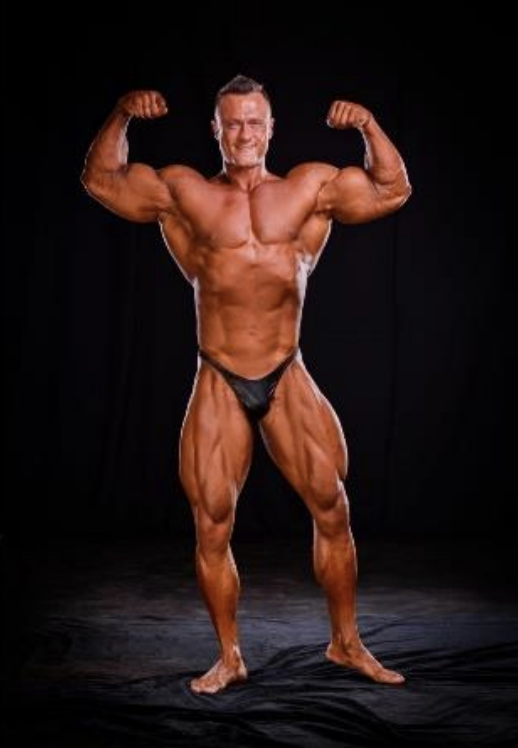
\includegraphics[width=0.75\linewidth, height=5cm]{figures/double_biceps.png}
            \caption{フロントダブルバイセップス}
            \label{fig:double_biceps}
        \end{minipage} &
        \begin{minipage}[t]{.33\textwidth}
            \centering
            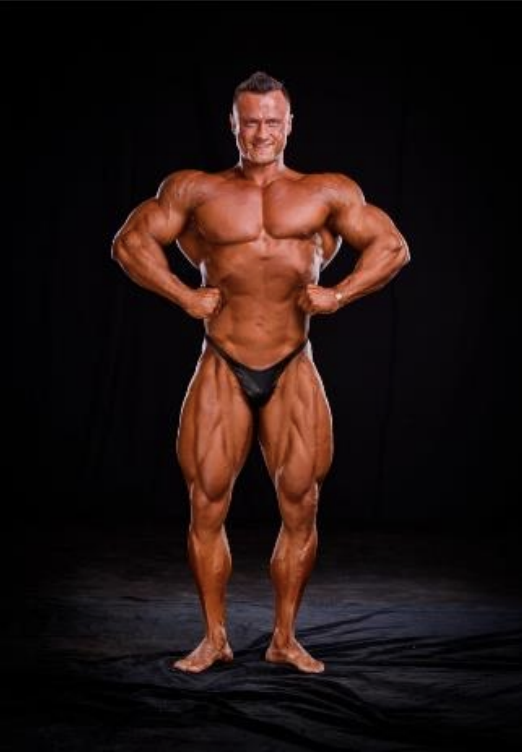
\includegraphics[width=0.75\linewidth, height=5cm]{figures/front_lat_spread.png}
            \caption{フロントラットスプレッド}
            \label{fig:front_lat_spread}
        \end{minipage} &
        \begin{minipage}[t]{.33\textwidth}
            \centering
            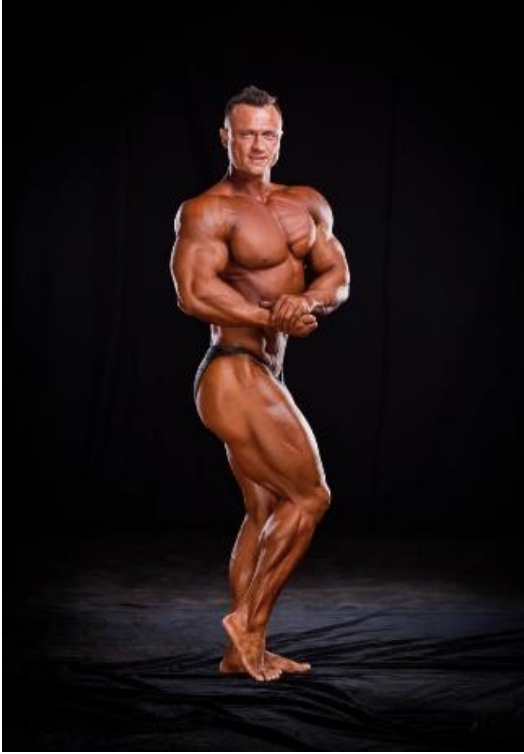
\includegraphics[width=0.75\linewidth, height=5cm]{figures/side_chest.png}
            \caption{サイドチェスト}
            \label{fig:side_chest}
        \end{minipage}
    \end{tabular}

    \begin{tabular}{cccc}
        \begin{minipage}{.25\textwidth}
            \centering
            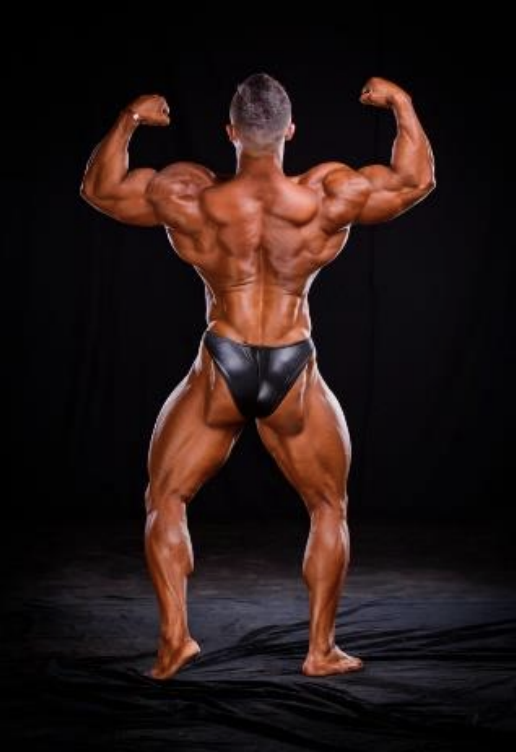
\includegraphics[width=0.75\linewidth, height=3.75cm]{figures/back_double_biceps.png}
            \caption{バックダブルバイセップス}
            \label{fig:back_double_biceps}
        \end{minipage} &
        \begin{minipage}{.25\textwidth}
            \centering
            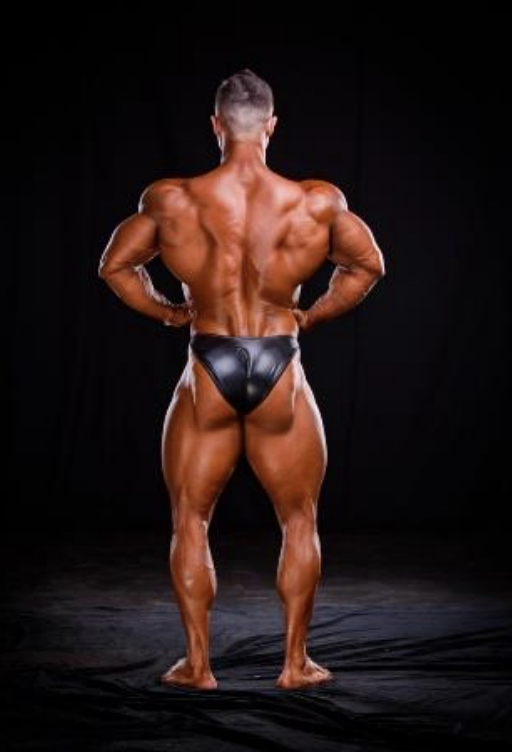
\includegraphics[width=0.75\linewidth, height=3.75cm]{figures/back_lat_spread.png}
            \caption{バックラットスプレッド}
            \label{fig:back_lat_spread}
        \end{minipage} &
        \begin{minipage}{.25\textwidth}
            \centering
            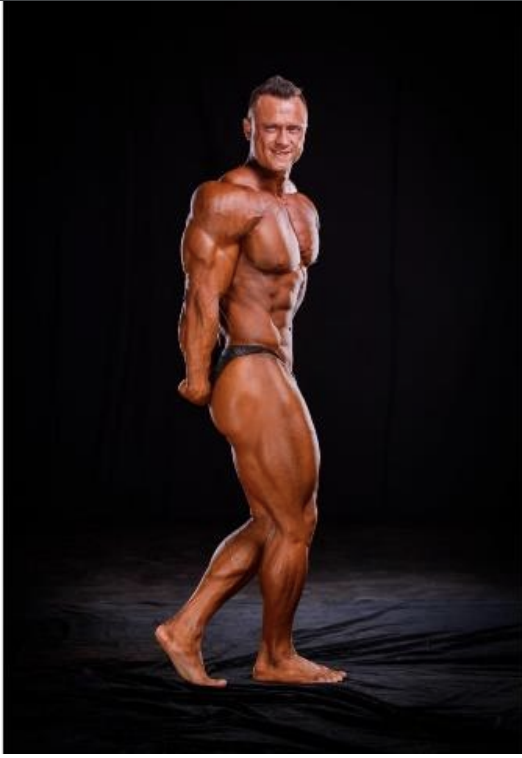
\includegraphics[width=0.75\linewidth, height=3.75cm]{figures/side_triceps.png}
            \caption{サイドトライセップス}
            \label{fig:side_triceps}
        \end{minipage} &
        \begin{minipage}{.25\textwidth}
            \centering
            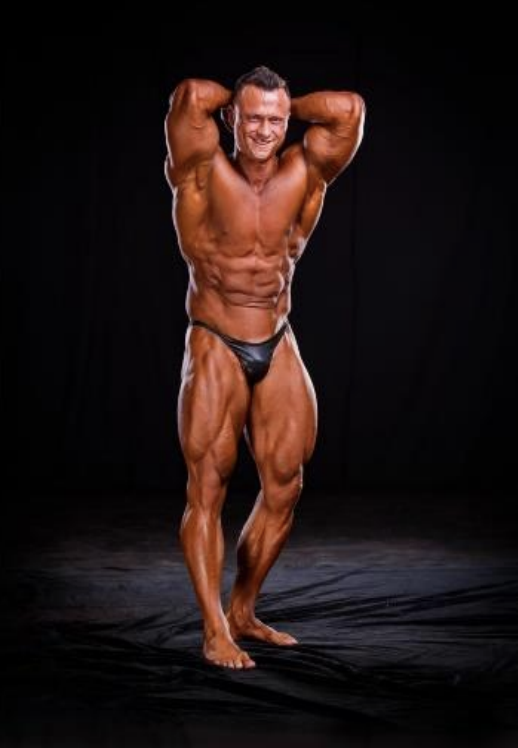
\includegraphics[width=0.75\linewidth, height=3.75cm]{figures/abdominal_and_sai.png}
            \caption{アブドミナルアンドサイ}
            \label{fig:abdominal_and_sai}
        \end{minipage}
    \end{tabular}
\end{figure}



の7ポーズである。この規定ポーズと前後左右のリラックスポーズで比較審査が行われる。

ポージングはボディビルにおいて大会当日にできる唯一の要素であり、鍛え上げてきた肉体をより良く見せるための重要なものである。しかしながら、ポージングはトレーニングの使用重量や、減量時の体重の変化といった指標となるものがない。
そのため初心者においてはトレーニングや減量を優先することが多く、ポージング練習の優先度が低い傾向にある。また、ポージングにおいては他者からのフィードバックがあることが望ましく、競技者の知り合い等がいない場合はパーソナルトレーナーなどから指導を受けることがあるが、
その場合は費用や時間の問題から初心者が何度も通うことはハードルが高い。

\section{ボディビルにおけるポージングの重要性}
JBBFにおけるボディビルの審査基準はJBBF競技マニュアルのメンズボディビル審査ポイントで以下のように定められている\cite{JBBF2023}。

\begin{enumerate}
  \item 究極の筋肉美
  \item 各部位の筋肉量
  \item 各部位のボリューム
  \item 各部位の密度
  \item 仕上がりのハードさ
  \item 上半身下半身左右のバランス
  \item ポージングセンス
  \item フリーポーズでの芸術性・表現力
  \item コスチュームの着こなし・身だしなみ
\end{enumerate}
このように、ポージングセンスは複数ある審査基準の一つであるが、他の審査基準で挙げられている肉体の完成度を見る項目をよりよくはっきするためには大切である。
ポージングはボディビルにおいて大会当日にできる唯一の要素であり、ポージングによって弱点を隠すことや、逆に強みをより活かすことができる。


\section{骨格推定}
骨格推定とは深層学習などを用いて人物のポーズを可視化してくれる手法であり、モーションキャプチャーなどの機器を使用することなく,
画像、動画データ、又はカメラからの入力を用いて人間のポーズを可視化することができる。
カーネギーメロン大学(CMU)の Zhe Caoら が「Realtime Multi-Person pose estimation」\cite{openpose}の論文で発表した、OpenPoseが一つの例である。\ref{fig:openpose}
骨格推定はさまざまなスポーツへ利用されている。上智大学大学院の金子ら \cite{soccer_openpose}はOpenPoseを用いてサッカーのシュートフォームを取得し、体の傾き、軸足、腰の回転、フォロースルーを特長量として用い、習熟度ごとに分類を行った。
TODO:もう少し骨格推定の応用例を増やす。
\begin{figure}[htbp]
    \begin{center}
        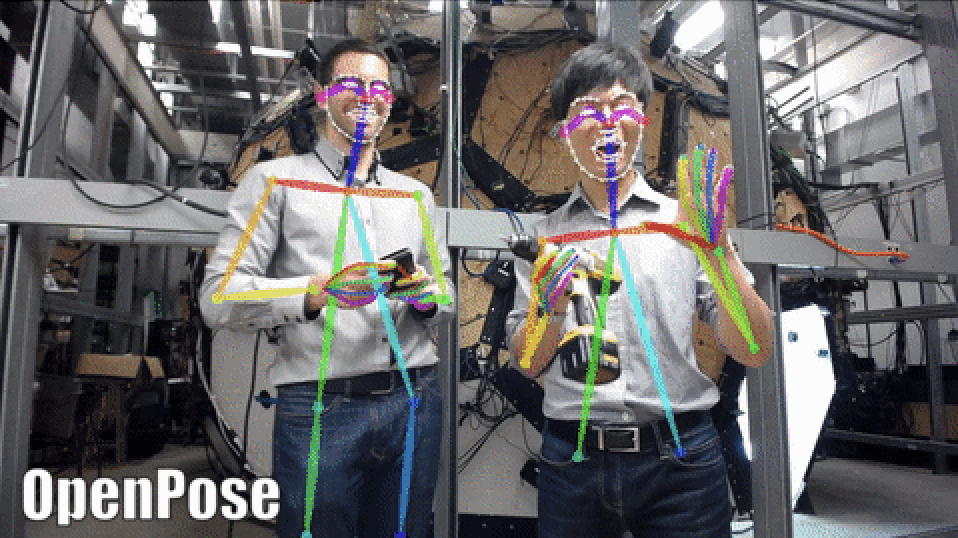
\includegraphics[width=7cm]{figures/openpose.png}
        \caption{OpenPose}
        \label{fig:openpose}
    \end{center}
  \end{figure}
\section{ガイダンス仮説}
ガイダンス仮説\cite{guidance_hypothesis}とは、フィードバックの頻度に関する仮説であり、学習中全ての試行においてフィードバックを与えると学習者はフィードバックに依存してしまい、
その結果、フィードバックを伴う練習中においてはパフォーマンスが優れているものの、フィードバックがない保持テストでは正確な運動を行えないことが多い。これは外在的フィードバックに依存してしまい、内在的フィードバックをおろそかにしてしまうためであると考えられている。
ここでいう内在的フィードバックとは、
私たちが動作を実行する際に自分の感覚に基づいてその動作を評価し、学習するプロセスである。
例えば、歩行時に足の裏から伝わる路面の感覚を認識することや、自分の進む方向を視覚的に確認することも、この内在的フィードバックの一例であることと言える。\cite{nagoyahml_feedback}
TODO: フィードバック周りの背景を増やす

ガイダンス仮説提唱後、フィードバックの与え方については様々な研究がなされている。ガイダンス仮説の否定的な効果を軽減するために、フィードバックの頻度を減らすことでフィードバックへの依存を減らす方法が提案されている。
それ以外にも、フィードバックの回数をだんだんと減らしていく漸減式フィードバック(Faded feedback)\cite{Aoyagi2019}や複数の試行の平均のフィードバックを与える平均化フィードバック(Averaged feedback)\cite{Aoyagi2019}などがある。
